%% line1.tex
\documentclass{standalone}
\usepackage{tkz-euclide}
\usetkzobj{all}
%% ================== commands ==========================
\newcommand{\myShowPoints}[2]{
\tkzDrawPoints(#1) 
\tkzLabelPoints[#2](#1)
}		
\newcommand{\myGetMidPoint}[3]{
\tkzDefMidPoint(#1,#2)\tkzGetPoint{#3}
}		
\begin{document}
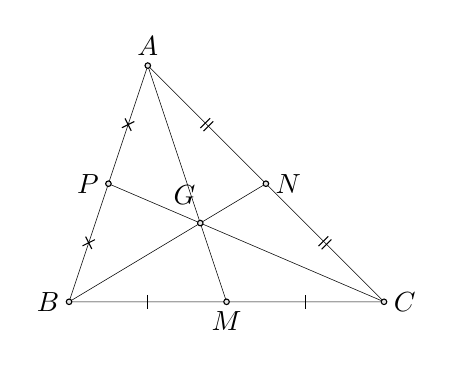
\begin{tikzpicture}

	\tkzDefPoints{0/0/B, 4/0/C, 1/3/A}
	% connecting 3 points
	\tkzDrawPolygon(A,B,C)
	
	\tkzCentroid(A,B,C)\tkzGetPoint{G}
	\tkzDrawLines[add = 0 and 1/2](A,G B,G C,G)


	\tkzLabelPoints[right](C)
	\tkzLabelPoints[above](A)
	\tkzLabelPoints[left](B)
	\tkzLabelPoints[yshift=6mm, xshift=-2mm](G)


	\coordinate (M) at ($(B)!.5!(C)$);
	\coordinate (N) at ($(A)!.5!(C)$);
	\coordinate (P) at ($(A)!.5!(B)$);
	\tkzMarkSegment[mark=|, size = 2.5](B,M)
	\tkzMarkSegment[mark=|, size = 2.5](C,M)
	\tkzMarkSegment[mark=||, size = 2.5](C,N)
	\tkzMarkSegment[mark=||, size = 2.5](A,N)
	\tkzMarkSegment[mark=x, size = 2.5](A,P)
	\tkzMarkSegment[mark=x, size = 2.5](B,P)
	\tkzDrawPoints(A,B,C,G,M,N,P)
	\tkzLabelPoints[below](M)
	\tkzLabelPoints[right](N)
	\tkzLabelPoints[left](P)
\end{tikzpicture}
\end{document}